% March 26, 2013
% Latex templete for preparation of Project Report of Final Year of MCA Students
%
% In Latex any command starting with % treated as comment.

% ------------------------------------------------------------------------------------
% Packages (if any package not installed on ur PC, just connect internet and run ur file, packages automatically installed)
% Document type and packages required (required package information is in etcreport.sty 
\documentclass[12pt, oneside, a4paper]{report}
\usepackage{etcreport}
\usepackage{titlesec}
\titleformat{\chapter}[display]
{\normalfont\huge\bfseries}{\filright\chaptertitlename\ \thechapter}{20pt}{\Huge\centering}

%-----------------------------------------------------------------------------------
\begin{document}
% ---------------------------------------------------------------------------------
% Add following chpaters - create separate tex files - sample files are given- edit them or create ur own
% ---------------------------------------------------------------------------------
\thispagestyle{empty}
  %\thisfancyput(3.25in,-4.5in){%
   %\setlength{\unitlength}{1in}\fancyoval(7,9.5)}

   \begin{center}
   \Huge \bfseries \textcolor{black} {A}\\[.2cm]
   \Huge \bfseries \textcolor{black} {Project Report}\\[.2cm]
	\Huge \bfseries \textcolor{black} {on}\\[.2cm]
% Change in following Line - Name of Project Title
% ---------------------------------------------------------------------
   \huge \bfseries \textcolor{purple} {``Digital India''}\\[.10cm]
   \Huge \bfseries \textcolor{black} {At}\\[.2cm]
   \Huge \bfseries \textcolor{black} {Krish Compusoft Services, Ahmedabad}\\[.9cm]
% ---------------------------------------------------------------------
   \large \bfseries \textcolor{black} {Submitted By:}\\[.2cm]
% Change in following Line - Name of Project Developer% -----------------------------------------------------------------
     \Large \bfseries \textcolor{purple} {Shubham K. Chaudhari}\\[.8cm]
     \Large \bfseries \textcolor{black} {To}\\[.2cm]
      
\includegraphics[scale=0.5]{Title/111}\\[0.1cm]
      \Large \bfseries \textcolor{cyan} { Institute of Management Research \& Development, Shirpur}\\[0.1cm]
  
      
% -----------------------------------------------------------------
   \Large \bfseries \textcolor{black} {North Maharashtra University, Jalgaon }\\[.7cm]
   \large \bfseries \textcolor{black} {Guided By:}\\[.2cm]

% Change in following Line - Name of Project Guide
% ---------------------------------------------------------------------
   \Large \bfseries \textcolor{purple} {Prof. Archana Jade.}\\[1cm]
% ---------------------------------------------------------------------
  
   \large \bfseries \textcolor{black} {  In the partial fulfillment of the requirement for the award of the degree of ‘Master of Computer Application’}\\[0.12cm]
   
   \huge \bfseries \textcolor{purple} {2021-22}\\[0.1cm]
\end{center}
 % add titlepage (stored in Title folder)
\thispagestyle{empty}
%\thisfancyput(3.25in,-4.5in){%
%\setlength{\unitlength}{1in}\fancyoval(7,9.5)}
\begin{center}

\includegraphics[scale=0.5]{Certi/111}\\[0.1cm]
\normalsize \bfseries \textcolor{black} {R. C. Patel Educational Trust's}\\[0.1cm]
\LARGE \bfseries \textcolor{cyan} {R. C. Patel Institute of Managment Research \& Development }\\[0.1cm]
\large \bfseries \textcolor{black} {Shirpur, Dist-Dhule 425405}\\[0.1cm]
----------------------------------------------------------------------------- \\[0.9cm]

\underline{\textit{\LARGE \textcolor{purple} {CERTIFICATE}}}\\[0.1cm]
\end{center}
\begin{flushleft}
\justifying
\begin{spacing}{2}
% Change in following Lines - Write ur Project Title, Names of Project Group Members  
% ---------------------------------------------------------------------------------


\textit{\large \textcolor{black}  This is to certify that Mr. Shubham K. Chaudhari, a final year student of \textbf {'Master of Computer Application'} from Institute of Management Research \& Development, Shirpur has successfully completed the project enttled \textbf{``Digital India''} as a part of academic six month industrial training which is approved for degree of Master of Computer Application a post graduate course of \textbf {'North Maharashtra University, Jalgaon'} during acadmic year 2021-22.}   \\[0.9cm]


 %---------------------------------------------------------------------------------
\end{spacing}
\noindent
%Date:\\[0.3cm]
%Place: Shirpur\\[1.6 cm] 
\textbf{Director \hspace{9cm} Examiner\\RCPETS IMRD,\\ Shirpur}\\[1.5cm]
%\textbf{ Exa}\hspace{5.5cm} %\textbf{Examiner}
\end{flushleft}
% End of Certificate	% add Certificate (stored in Certi folder)
\thispagestyle{empty}
%\thisfancyput(3.25in,-4.5in){%
%\setlength{\unitlength}{1in}\fancyoval(7,9.5)}
\begin{center}

\includegraphics[scale=0.5]{Certi/111}\\[0.1cm]
\normalsize \bfseries \textcolor{black} {R. C. Patel Educational Trust's}\\[0.1cm]
\LARGE \bfseries \textcolor{cyan} {R. C. Patel Institute of Managment Research \& Development }\\[0.1cm]
\large \bfseries \textcolor{black} {Shirpur, Dist-Dhule 425405}\\[0.1cm]
----------------------------------------------------------------------------- \\[0.9cm]

\underline{\textit{\LARGE \textcolor{purple} {CERTIFICATE}}}\\[0.1cm]
\end{center}
\begin{flushleft}
\justifying
\begin{spacing}{2}
% Change in following Lines - Write ur Project Title, Names of Project Group Members  
% ---------------------------------------------------------------------------------


\textit{\large \textcolor{black}  This is to certify that Mr. Shubham K. Chaudhari, a final year student of \textbf {'Master of Computer Application'} from Institute of Management Research \& Development, Shirpur has successfully completed the project enttled \textbf{``Digital India''} as a part of academic six month industrial training which is approved for degree of Master of Computer Application a post graduate course of \textbf {'North Maharashtra University, Jalgaon'} during acadmic year 2021-22.}   \\[0.9cm]


 %---------------------------------------------------------------------------------
\end{spacing}
\noindent
%Date:\\[0.3cm]
%Place: Shirpur\\[1.6 cm] 
\textbf{Director \hspace{9cm} Examiner\\RCPETS IMRD,\\ Shirpur}\\[1.5cm]
%\textbf{ Exa}\hspace{5.5cm} %\textbf{Examiner}
\end{flushleft}
% End of Certificate	% add Certificate (stored in Certi folder)
\thispagestyle{empty}
\begin{flushright}
\textit{\Large \textcolor{black} Acknowledgement}\
\rule{6in}{.1pt}\\[0.5cm]
\end{flushright}
\justifying
\begin{spacing}{1.5}
% Change following - write ur acknowledgement (sample is given u may use same.
% ---------------------------------------------------------------------------------
I take this opportunity to express my sincere thanks to Krish Compusoft Services, Ahmedabad for provideing me an opportunity to work in the organization. I also express my gratitude to \textbf{ Mr. Mahipal Likhiya(Technical Head)} Krish Compusoft Services, Ahmedabad who gave me the opportunity to work in Krish Compusoft Services. His prudent ideas of work, keen interest in developing the system and constant effort were a great source of inspiration for us me. He not only guided us on the technical aspect but his acknowledgement of marketing strategies helped us in broadening our prespective.\\
	 I express my thanks to \textbf {Mr. Mahipal Likhiya (Team Leader)}. for their valuable guidance and experienced suggestion, encouragement and support extended by them helped me in various stages where I needed help and suggestions.\\
	 I am thankful to \textbf{Dr. Vaishali Patil. (Director), Prof. M. N. Behere (Head Dept. of MCA), and Prof. Archana Jade (Project Guide),  } R. C. Patel Institute of Management Research and Development, Shirpur, for giving me his valuable guidance and encouragement during our course. I am thankful to the college staff for their constant encouragement.\\
	 Last but not least, I am thankful to all people who directly or indirectly contributed to make this project a sucess.\\
	%We would be failing in our duties if we do not make a mention of our family members including our parents for providing moral support, without which this work would not have been completed.%

	
 	
	
	
% Change in following Line - Name of Project Group members     
% -----------------------------------------------------------------
\begin{flushright}
\begin{spacing}{1}
\textbf{Thanks \& Regards}\\[.03cm]
\textbf{Chaudhari Shubham K.}\\[.01cm]

\end{spacing}
\end{flushright}
\end{spacing}

 % add acknowledgement (stored in Ack folder)
%\thispagestyle{empty}
\begin{flushright}
\textit{\Large \textcolor{black} Abstract}\
\rule{6in}{.1pt}\\[0.5cm]
\end{flushright}
\justifying
\begin{spacing}{1.5}
Now a days, blind people can do more than anyone can Imagine. They can perform many computer applications, read textbooks and magazines, search on the Internet and send email. Some of the blind even can work as a clerk in office. Many different kinds of electronic devices are primarily designed for them in order to help them do whatever a normal person can do. The more popular and useful is the Braille display, which can display any text appearing on the computer to the blind user. Likewise Portable Braille Reader and Writer performs the job of reading and writing simultaneously. \\            
           This project will perform the functions such as  by using Braille keypad they can write any text and store the text into EEPROM. Also while writing it will provide sound of given text or word written. Text which has been written can be heard by blind user at any time. The document which is written can be uploaded on computer at any time using serial communication using RS232. Document which is present on computer can be uploaded on EPROM and can be heard at any time.\\                           
           There are many electronic models of Braille displays and writers available in markets. They all have one similarity, the cost. The price of the Braille displays in nowadays market is very high. These high costs are caused by two reasons, the invention of voice recognition and the smaller market size. Since the cost of the Braille displays is not affordable by many blind users, one of main goals is to build this device with low cost. Because this device  is built for a blind user, the focus of this project is to make the Braille unit and portable and user friendly.
\end{spacing}		% add abstract (stored in Abs folder)
% ---------------------------------------------------------------------------------
\renewcommand{\baselinestretch}{1.5}
\setlength{\textheight}{9.0 in} \setlength{\textwidth}{6in}
%\addtolength{\leftmargin}{-.3in} \topmargin -.2in \pagenumbering{}
\pagenumbering{roman}
\tableofcontents
%\cleardoublepage \addcontentsline{toc}{chapter}{List of Figures}
%\listoffigures
%\cleardoublepage\addcontentsline{toc}{chapter}{List of Tables}
%\listoftables
% ---------------------------------------------------------------------------------
% Add following chapters - create separate tex files - sample files are given- edit them or create ur own
% Chapter 1 - Introduction
% Chapter 2 - Basic Concept and Literature Survey
% Chapter 3 - Arrange as per ur project 
% Chapter 4 - Arrange as per ur project 
% Chapter 5 - Arrange as per ur project 
% Simmilarly last three chapters must be as per following:
% Chapter 6 - Testing Results
% Chapter 7 - Conclusion & Future Scope 
% Chapter 8 - References
% ---------------------------------------------------------------------------------
% for Figure insertion
% 		\begin{figure}[ht!]
%		\begin{center}					% for aligning figure, left center or right
%		\includegraphics[scale=3]{toplevelblock}  %add figure in eps / jpeg format
%		\caption{Top Level Block Diagram}  % name of figure to be displayed below 												   % figure and in List of figure
%		\label{fig:Block}		% for calling figure no. in text 
%								example  Figure ~\ref{fig:Block} which add figure no 									% automatically
%		\end{center}
%		\end{figure}
% If jpeg file not included (if Latex gives error) include eps file.
% u may convert jpeg file to eps by using software image converter plus, or u may convert online. 	
% ---------------------------------------------------------------------------------
\cleardoublepage \pagenumbering{arabic}
\pagestyle{fancy}
\lhead{\small \textbf{}}
\chead{}
\rhead{\small \textbf{PsfA}}
%\rhead{\includegraphics[height=0.8cm,width=1.6cm]{dcr24.jpg}}

\lfoot{\small \textbf {}}
\cfoot{}
\rfoot{\thepage}
\renewcommand{\headrulewidth}{.1pt}
\renewcommand{\footrulewidth}{.3pt}
\justifying

\begin{spacing}{1.5}
% ---------------------------------------------------------------------------------
% Add following chapters - create separate tex files - sample files are given- edit them or create ur own
\chapter{Introduction}



\section{Company Profile}

At KCS, as a cloud and data solutions company with expertise on various technology
platforms, we enable our global customers to achieve digital transformation and provide
smart product solutions with our tech consulting, bespoke solutions, as well as
professional services. We enable clients across the globe to navigate their digital journey
with integrated technology models, business intelligence, and next-gen tech expertise to
catalyze change.
Our pragmatic approach to technology with agile methodologies helps deliver
unprecedented levels of solutions, service performances and customer delight. With
almost two decades of experience and more than 80% of referral business, we have
delivered with process discipline while following CMMI Level 5, ISO 27001 standards
and partnering with Microsoft Gold partner, Google cloud partner, Amazon cloud partner
as well as other OEMs

% Student write your company profile

\subsection{ Services Offered }
\subsubsection{International Consultancy}
We have been providing international consultancy from last 22 years and during we have established competitive foundation. Our consultancy Service consists of a highly skilled.

% This section type your project contents 


\subsubsection{Technical Consultancy}
Be it B2B, B2C or even B2E, KCS has driven service-centric project engagement models and have executed various end to end IT strategies including concept planning, architecture planning, project management, infrastructure planning, resource planning, applications development, database management, IT infrastructure planning and management, training as well as deployment. Our offerings include the
entire gamut from IT strategies to application development services.

% This section type your project contents 


\subsubsection{Web Development }
Today, the major increasing internal efficiencies and productivity through web services. We target that 

tools Our development team is well versed with the and technologies like- PHP, ASP .Net, Javascript, Ajax, React, NodeJs and Angular.

% This section type your project contents 

% This section type your project contents 
\subsubsection{Web Hosting }
The important and most overlooked aspect of site development is hosting. We offer reliable, secure and super-fast hosting services. We also provide hosting solutions.

% This section type your project contents 

\subsubsection{Software Development }
We are strong believers that the software you use for your business should be designed around.
% This section type your project contents  

\subsection{Clients and Products}
\begin{itemize} 


\item	Smart Town Mobile App. 
\item	eHospitality Services Management(eHSM) .
\item	H-Connect (Connecting Health Globally).
\item	\textbf{Digital India. }\\
          Website: http://www.kcsitglobal.com 
      
\end{itemize}




\section{Introduction To Digital India }
                             Digital India is a Web Application built using MERN (MongoDB, Express, React,
NodeJS) Stack. With Digital India you can register the electronic devices and control is
via Single Dashboard from anywhere.
It uses IoT Technology to achieve this functionality
                             .
\subsection{Need And Motivation}

% This section type your project contents 

\textbullet \hspace{0.2cm}The home automation market is primarily driven by growing need for effective solutions
in various domestic applications such as lighting, safety and security, energy
management, entertainment, and HVAC (heating, ventilation, and air conditioning).


\subsection{Problem Definition }
The project aims to design and construct a home automation system that Will remotely switch on or off any household appliances connected to it, using a microcontroller, voice dial on a phone, or Bluetooth/-based android application.
% This section type your project contents 

\subsection{Objective And Scope}
Considering the problem project is to develop Digitaly control Light,Fan,Tv etc. -  \textbf{Digital India}\\Application such that it overcomes the flaws of existing manual Switch. 
	 .\\
\textbullet \hspace{0.2cm}	\textbf{Device Owner}\\
o	Can add, update and delete new users and assign proper roles to them in the User concerned.  \\
o	User can  and to Add Device to Whitelist specific Command.\\

% This section type your project contents 

\subsection{Features of Proposed System}
Digital India systems involve making homes even smarter. Homes can be interfaced with sensors including motion sensors, light sensors and temperature sensors and provide
automated toggling of devices based on conditions.

\textbullet \hspace{0.2cm}Ability to control any registered device from a single dashboard.\\
\textbullet \hspace{0.2cm} Ability to register various type of devices that can be controlled later on using
commands \\
\textbullet \hspace{0.2cm}Ability to register different commands to control the registered devices \\
\textbullet \hspace{0.2cm} Ability to connect Google Assistant and Alexa to control the registered devices


% This section type your project contents 
 % include ur chapter introduction in report.
\chapter{System Requirement Analysis}


\section{System Requirement Analysis}
At system requirement analysis stage the information gathering process is identified a Smart devices fueled by the hyper-connected Internet of Things (IoT) are becoming
ever more prevalent and pervasive in our personal lives. Sensors are everywhere, and the trend will only continue. Today, sensor-equipped industrial equipment is powered by artificial intelligence (AI). Medical devices can self-diagnose and send alerts to patients and doctors to remotely manage healthcare. Automobiles with in-car connectivity can download new features on the fly. Very soon, refrigerators will plan your dinner and ovens will know how to cook it.


%\begin{itemize} 

%\item Generate  the  bill  for  the  user  and  enter  it  in  the  database.
%\item Over the counter charge management.
%\item Preparation of monthly reports.
%\item Status of the parcel.
%\item Built in backup and restore facilities.
%\item hhghfhgh
%\item Trace out the parcel.

%\end{itemize}


\section{Software Process and Development}
The set of general objectives for "Digital India" development were defined by the various \\
% This section type your project contents 
\textbf{Prototype model}\\

The prototyping paradigm begins with requirements gathering. Together with Panning of those aspects of the software that will be visible to the customer/user (e.g. input approaches and output formats).

% This section type your project contents 

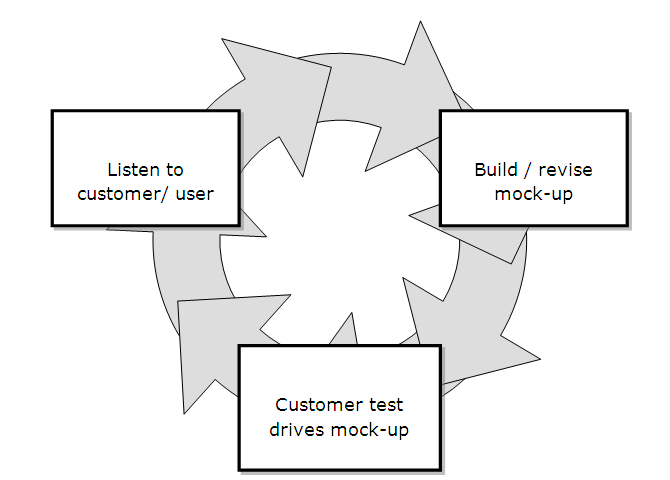
\includegraphics[scale=0.8]{Ch2/prototype.png}

\label{fig:Prototype Model}

% Diagram change as per your project demands

\section{Scope of Proposed System}
Our main purpose is to create a MERN application that helps Customers and other people use their home appliances remotely using their remotely held devices like Mobile phones, tablets, etc.


%\section{Hardware & Software Specifications}


% Write scope of your system.

\section{Technical Specification}
\textbullet \hspace{0.2cm} \textbf{Server}\\
Processor	:	Intel i3\\
RAM          	: 	Min. 512 MB\\
Hard Disk	: 	Min. 512 MB free\\
\textbullet \hspace{0.2cm} \textbf{Client}\\
Processor   	: 	Intel i3 or Above\\
RAM           	: 	Min. 512 MB\\
Hard Disk	: 	Min. 480 MB free\\
\textbullet \hspace{0.2cm} \textbf{Software Specification}\\
Platform	:  	Windows XP\\
Front End	: 	HTML, JavaScript,CSS,React \\
Middle ware	: 	JavaScript,Express,Node\\
Back End	: 	MongoDB \\
Framework: Express\\	
Web Browser: 	Chrome etc. \\


\subsection{Express Framework}
Express is a NodeJS-driven framework, you churning out dynamic, interactive, professional websites in no time.\\

\textbullet \hspace{0.2cm}	It underpins the Model/View/Controller (MVC) approach to web development—a best practice philosophy all developers should adhere to.\\

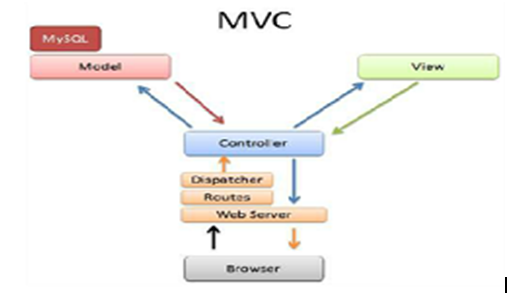
\includegraphics[scale=1.0]{Ch2/mvc.png}


% Diagram change as per your project demands (If required)
\label{fig:MVC Model}

%\textbullet \hspace{0.2cm}It’s built on a linear, easy-to-use folder structure.\\


% This section type your project contents 
\chapter{Feasibility Study}


\section{Introduction}
the working of the system, \\
Therefore, a feasibility study of the proposed system needs to be carried out in order to:\\
\textbullet \hspace{0.2cm} 	Provide a better understanding of the System.\\
\textbullet \hspace{0.2cm}	Describe the outputs.\\

There are many factors. These factors are \textbf{Economical Feasibility, Technical Feasibility and Operational Feasibility}.\\

% This section type your project contents 


\section{Economical Feasibility}
\textbullet \hspace{0.2cm}Economic Feasibility helps in determining whether the required software has the potential to generate financial gains for an organization.\\
\textbullet \hspace{0.2cm}The only person working here is an admin. So due to reduced manpower,the cost of wages is also reduced. Hence making it cheaper.\\

% This section type your project contents 
\section{Operational Feasibility}
\textbullet \hspace{0.2cm}The GUI is designed to be user friendly, so it is easy to use by admin. There is only one user which handles the website i.e., Admin. So, the manpower required is less here.\\
\textbullet \hspace{0.2cm}This software will have a very easy to use, user friendly interface so it will be pretty much operable by anyone having little experience with android or iOS phone.\\
\section{Financial and Economical Feasibility}
% This section type your project contents 
\textbullet \hspace{0.2cm}This type of study involves the cost incurred on the team of the software development, cost of study involved in conducting a feasibility study,
estimated cost of software and hardware.\\
\textbullet \hspace{0.2cm}Here the cost of hardware is affordable

\chapter{Proposed System}


\section{Proposed System}
helps to manage Electronic Equipment in Home.\\

\textbf{User Registration:} It provides Add User/Delete User/Give Specific Access on Electronic Divice.\\
% This section type your project contents
 
\textbf{Command Center:} In Command Center you can add commands ,Run commands and store command logs, It stores information .\\
% This section type your project contents 

\textbf{Authorize:} In this module Verify User using OTP Verification, Google Assistant and Alexa Authorizations.\\
% This section type your project contents 


\section{User Privileges}
The user type determines the privileges that the user has within Home. Two types of User as follow\\
\begin{itemize}
\item Device Owner(Mannage user,Mannage command)
\item Normal User(Run Command)
\end{itemize}

% This section type your project contents 

\section{Objective of the System}
% This section type your project contents 

\begin{itemize}
\item Latest technology 
\item Graphical user Interface
\item AI and IoT based System
\end{itemize}
\chapter{Preliminary  Design}

\section{Tools of data flow strategy}
	Data flow strategy shows th and their interactions.\\
\textbf{Data flow analysis makes use of the following tools:}\\
Flow Charts\\
Data Flow Diagrams\\
Data Dictionary\\
\textbf{Flowchart}\\
Flowchart is used to represent the algorithm.\\
\textbf{Data Dictionary}\\
The logical characteristics of current systems data stores, including name, description, aliases, contents.\\
\textbf{Data Structure Diagrams}\\
A pictorial description of the relation between entities (people, places, events and things) in system and the set of information about the entity.\\
\textbf{Structured Chart}\\
A design tool that pictorially shows the relation between processing modules in computer software, describes.


%-----------------------------------------------------------------

\section{Use Case Diagram}
%If you add information about use case diagram\\
\subsubsection{Usecase Diagram For User}
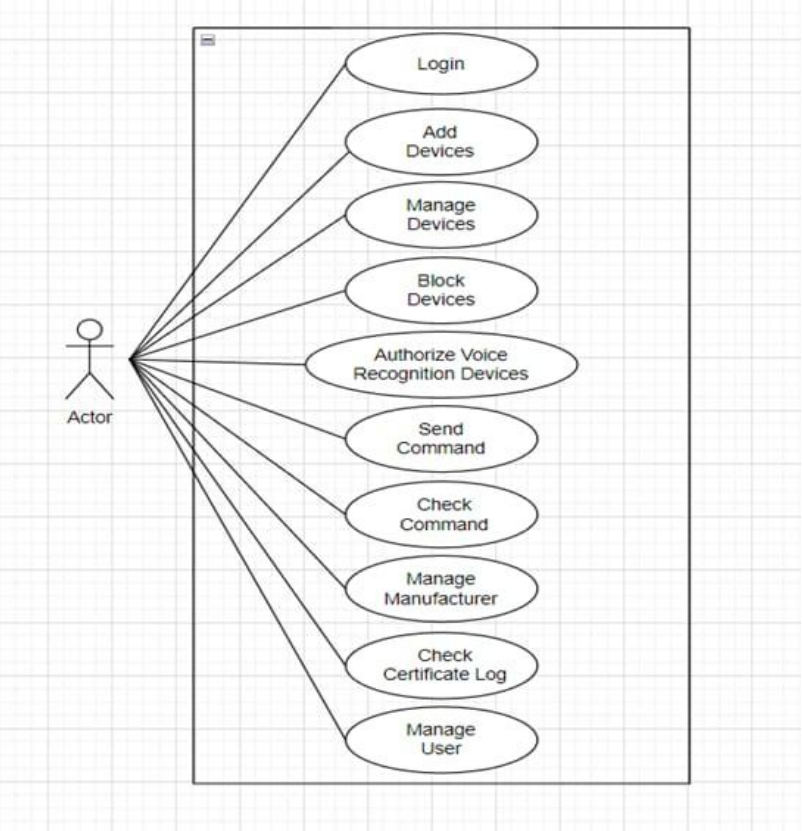
\includegraphics[scale=0.7]{Diag/usecaseadmin.png}

\label{fig:Use case diagram For User}






%-----------------------------------------------------------------
%\section{Activity Diagram}
%%If you add information about Activity Diagram\\
%
%\includegraphics[scale=.8]{Diag/activitylogin.png}
%\label{fig:Activity Diagram}



%-----------------------------------------------------------------

\section{Entity Relationship Diagram}

\subsubsection{ERD For User.}
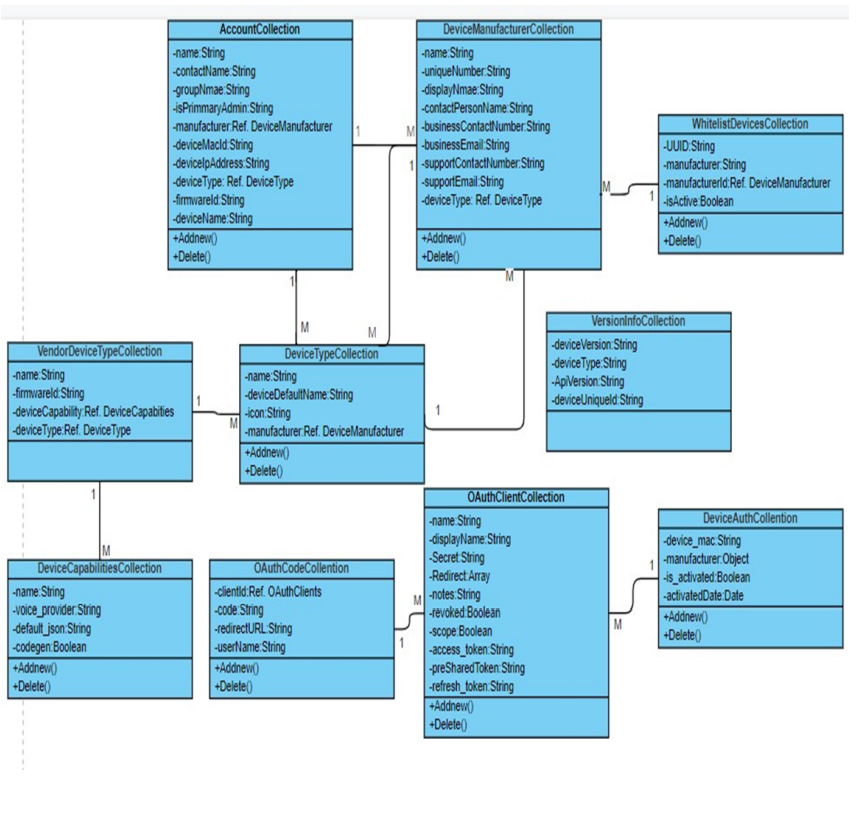
\includegraphics[scale=0.7]{Diag/ERDuser.png}
\label{abc}




%\subsubsection{ERD For users.}
%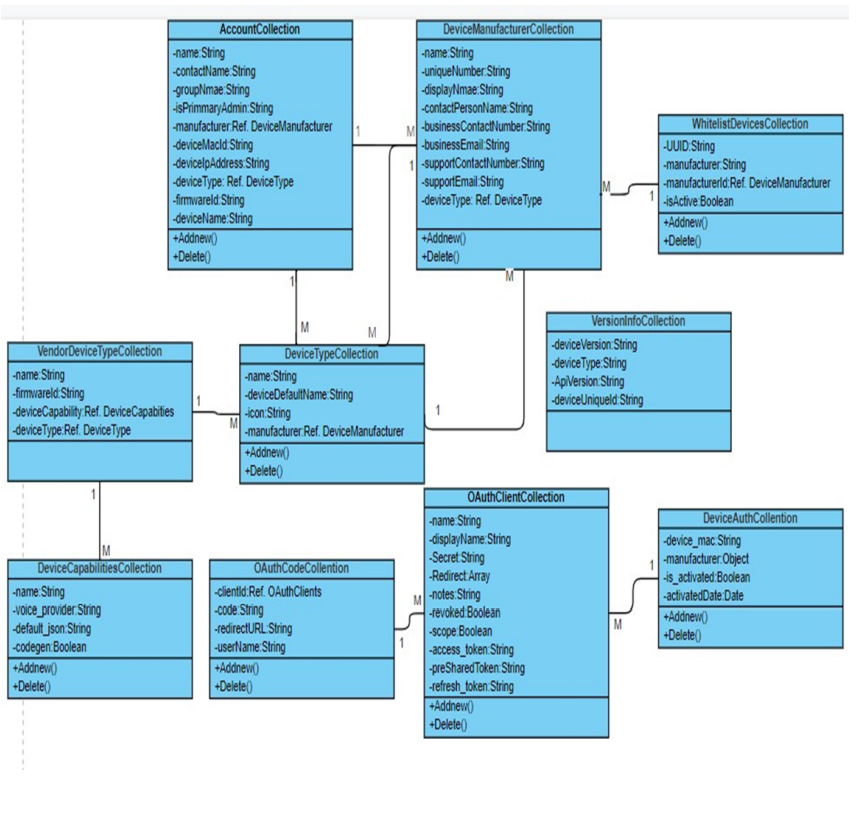
\includegraphics[scale=0.7]{Diag/ERDuser.png}
%\label{abc}
%
%\subsubsection{ERD For Products.}
%\includegraphics[scale=0.7]{Diag/ERDprod.png}
%\label{abc}
%-----------------------------------------------------------------

\section{Data Flow Diagram}
%If you add information about Data flow diagram\\

%\begin{figure} [h]
%\begin{center} 
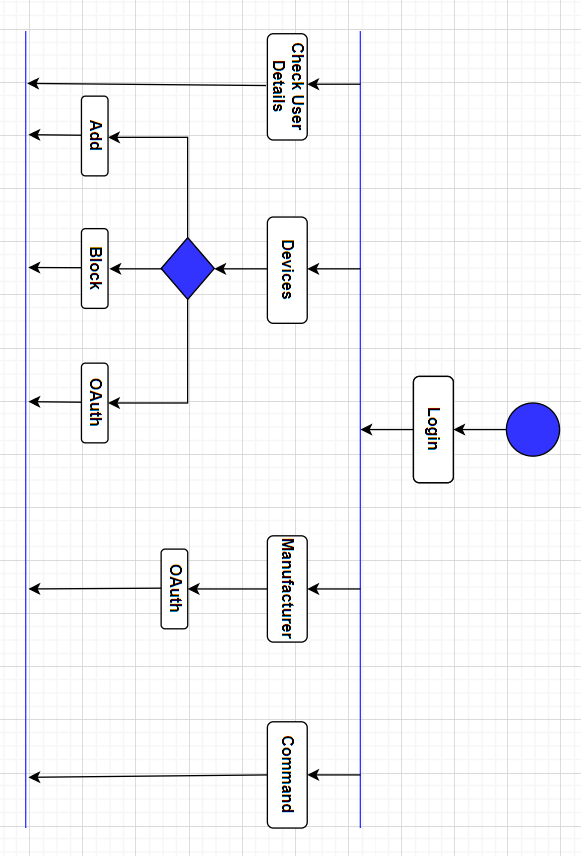
\includegraphics[scale=.9]{Diag/d1.png}
\label{fig:Contex Level}
%\end{center}
%\end{figure}

%\begin{figure} [h]
%\begin{center} 
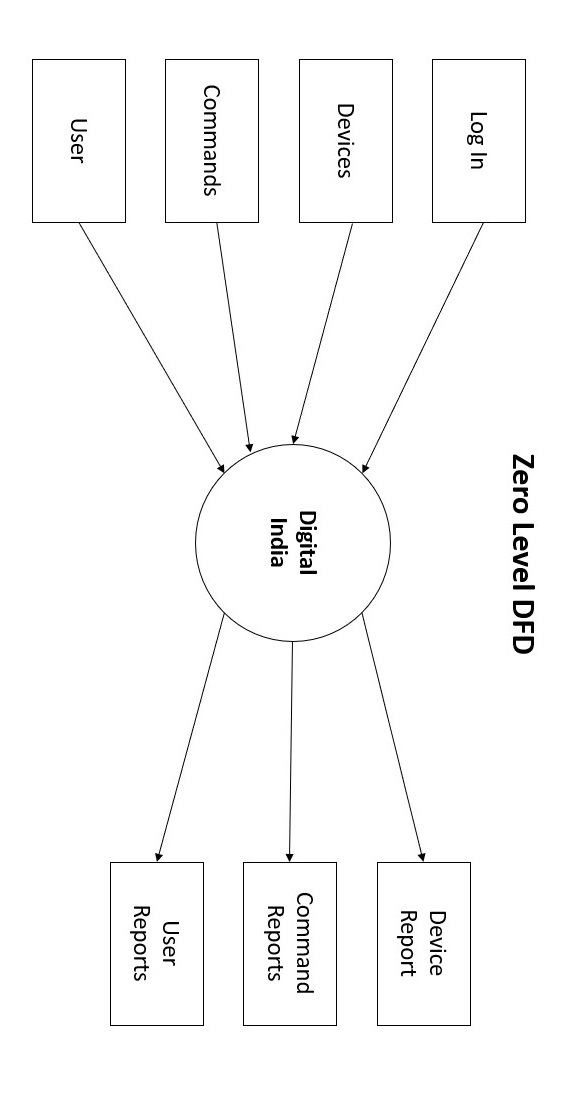
\includegraphics[scale=.9]{Diag/DFD_Zero.jpeg}
\label{fig:Contex Level}
%\end{center}
%\end{figure}

%\begin{figure} [h]
%\begin{center} 
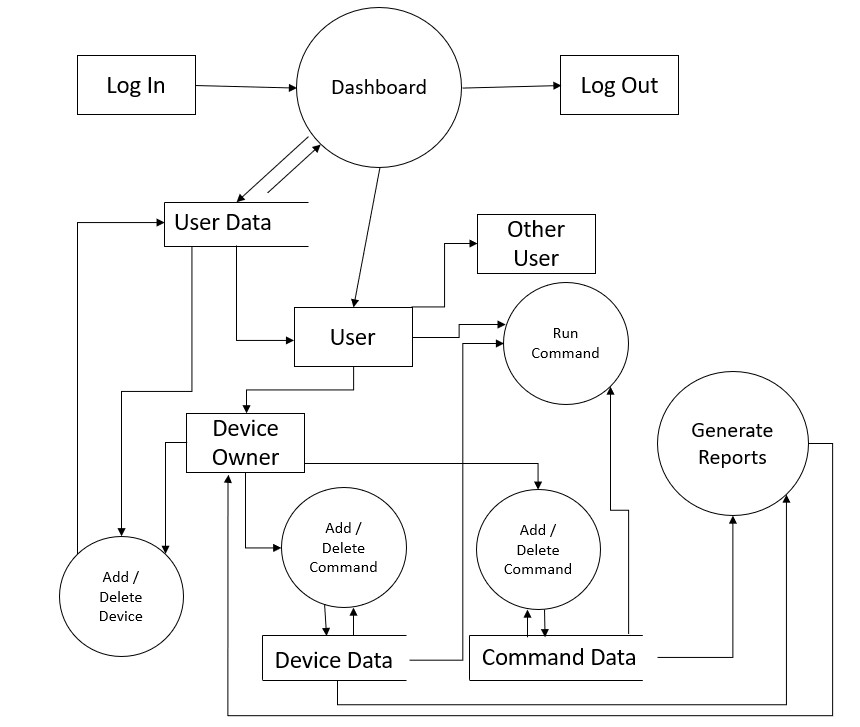
\includegraphics[scale=.9]{Diag/DFD_One.jpeg}
\label{fig:Contex Level}
%\end{center}
%\end{figure}



%\begin{figure} [h]
%\begin{center} 
%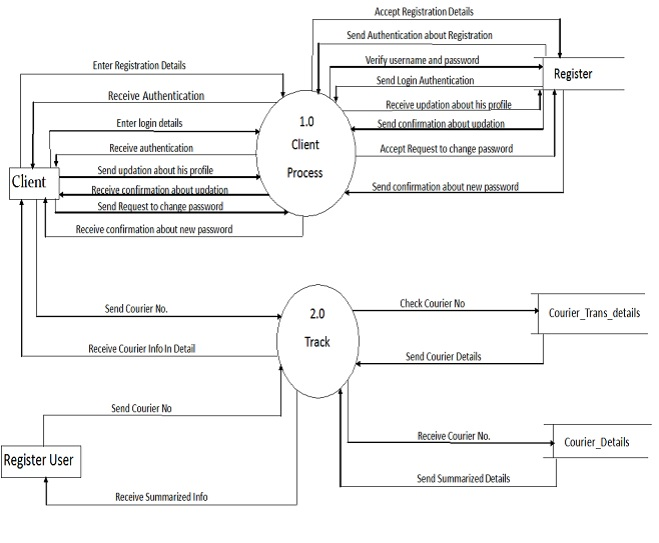
\includegraphics[scale=.9]{Ch5/dfd2.jpg}
%Fig. Data Flow Diagram
%\label{fig:DFD2}


\
% Students should divide chapter 3,4,5 according to major blocks of their project
\chapter{Detailed Design}

etailed design done by specifying algorithm and structure that makes up the interior modules. Usually there are many choice but from the different alternatives available. The one, which offer greatest efficiency, simply functionality is selected based on the relative important of these criteria

\section{Data Dictionary}
A data dictionary provides a complete documentation of all the element of system like data items, data stores(database) and data flow. Data described in data dictionary carries the details of the type, data name, database name, data description and characterization. Data Dictionary covers the whole organization or a database.
Data Dictionary is only collection of the element definition.

\section{Input and output Design}

		Considering all o the interaction of user with the system be in most effective and simplified way.                All the input forms are designed in she user will be able to use them in very eff possibilities needed by the user................
		
		
		% This section type your project contents 
		
		
		
\subsection{Admin}

\begin{center}
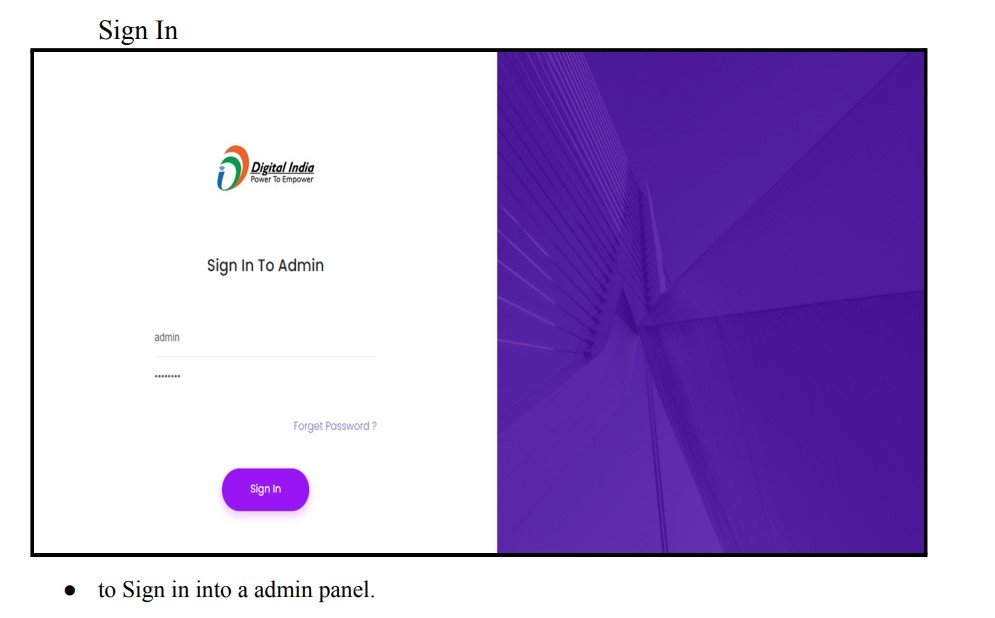
\includegraphics[height=9cm,width=14cm]{Admin/Sign.jpg}
\end{center}


% This section type your project contents 

\begin{center}
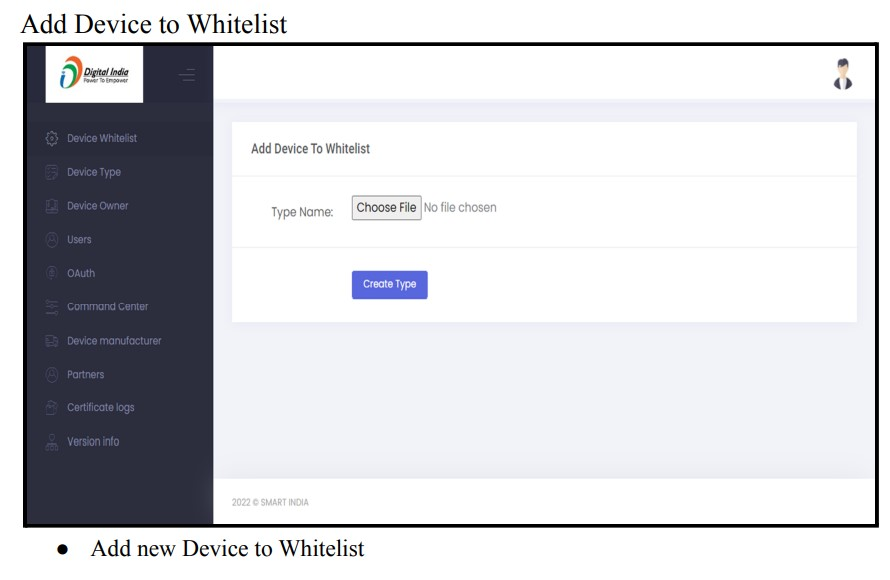
\includegraphics[height=9cm,width=14cm]{Admin/Addwhitelist.jpg}
\end{center}
\pagebreak


\begin{center}
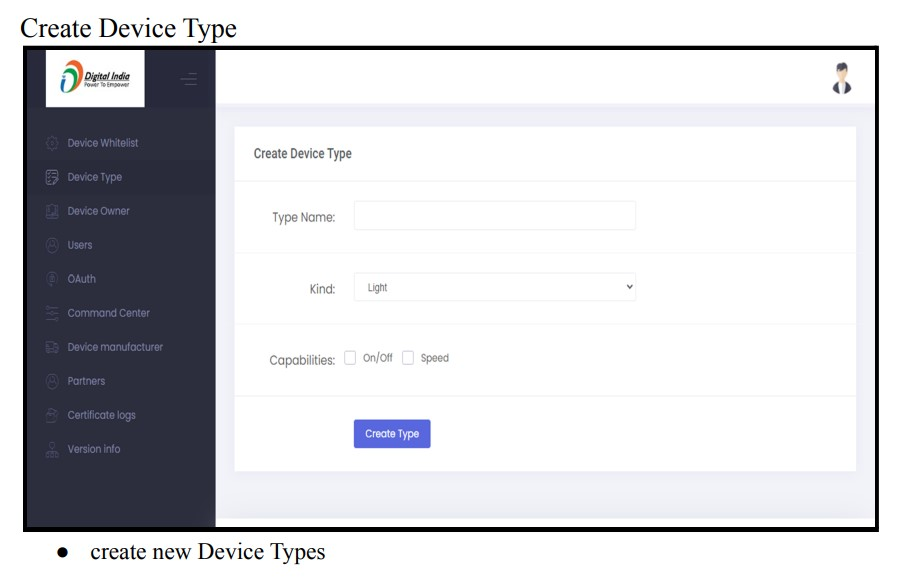
\includegraphics[height=9cm,width=14cm]{Admin/Adddivice.jpg}
\end{center}



% This section type your project contents 

\begin{center}
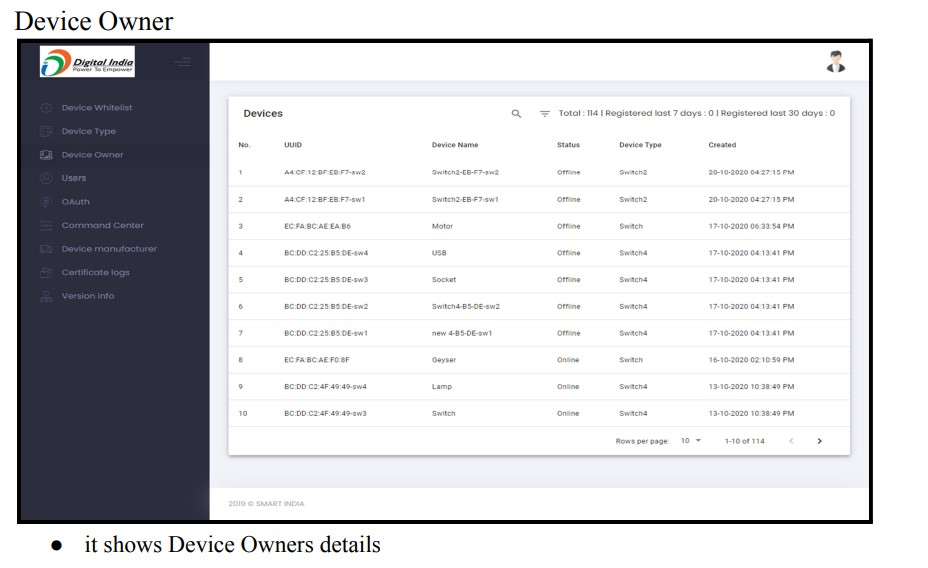
\includegraphics[height=9cm,width=14cm]{Admin/Deviceowner.jpg}
\end{center}
\pagebreak

\begin{center}
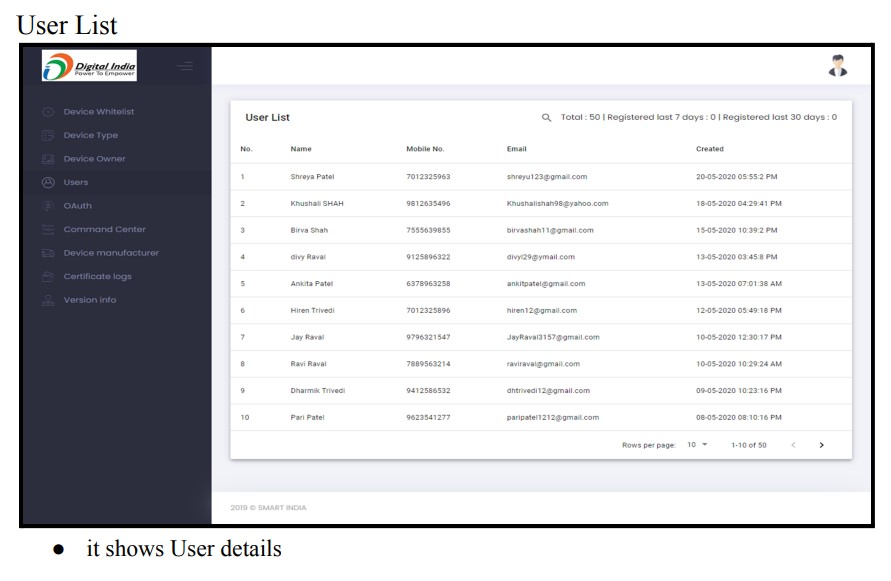
\includegraphics[height=9cm,width=14cm]{Admin/Userlist.jpg}
\end{center}

\begin{center}
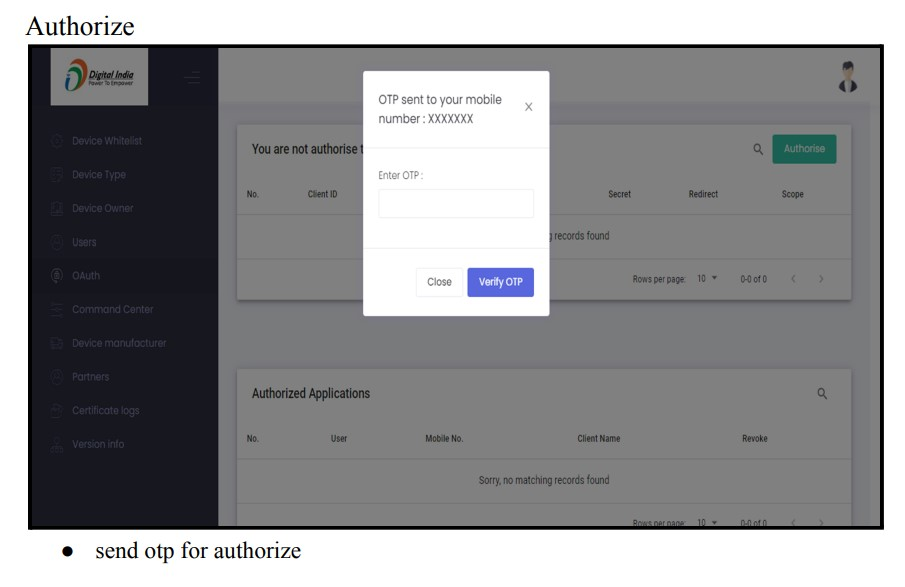
\includegraphics[height=9cm,width=14cm]{Admin/Authorize.jpg}
\end{center}
\pagebreak

\begin{center}
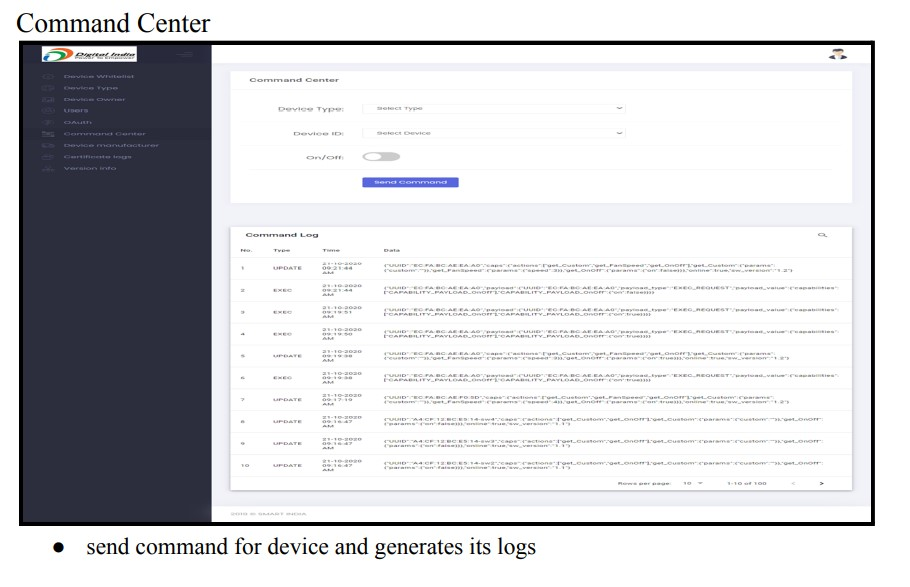
\includegraphics[height=9cm,width=14cm]{Admin/Commandcenter.jpg}
\end{center}

\begin{center}
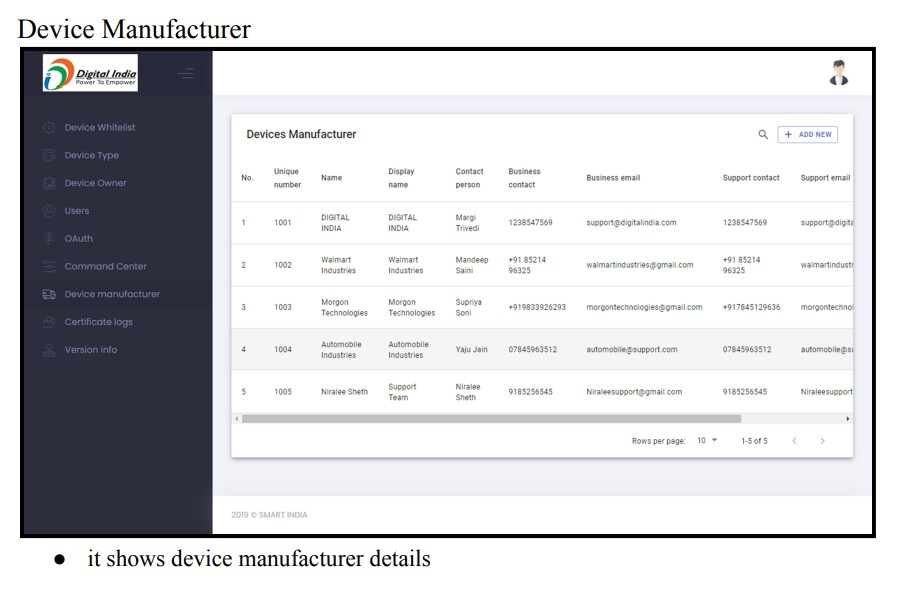
\includegraphics[height=9cm,width=14cm]{Admin/Device.jpg}
\end{center}
\pagebreak

		
		% This section type your project contents 
		
		
		
		
		
		
		
		
		
		
		
		
		
		
		
		
		
		
		
		
		
		
		
		
		
		
		
 		

\section{Database structure}
\textbf{Account Collection:}  This table stores Information for Creating account and give access to login.\nolinebreak
\begin{table}[hp]
\centering

\begin{tabular}{|c|c|c|c|}
\hline
\textbf{Field Name}  & \textbf{Data Type}  & \textbf{size} &\textbf{Constraints}  \\
\hline
name & String & 50 & NOT NULL \\
\hline
contactName &	String &	50 & NOT NULL\\
\hline
groupName & String &	50 & NOT NULL\\
\hline
isPrimaryAdmin	& Boolean & - &	NOT NULL\\
\hline
manufacturer &	Object &	- &	-\\
\hline
deviceMacId &	String & 30 &	NOT NULL\\
\hline
deviceIpAddress & String & 30 & NOT NULL\\
\hline
deviceType	& Object &	- & - \\
\hline
firmwareId	& String &	20 & NOT NULL \\
\hline
deviceName	& String &	20 & NOT NULL \\
\hline

\end{tabular}
\caption{ Account Collection}
\end{table}
\\
\textbf{Command Collection:} This table stores Commands .\nolinebreak
\begin{table}[hp]
\centering
\begin{tabular}{|c|c|c|c|}
\hline
\textbf{Field Name}  & \textbf{Data Type}  & \textbf{size} &\textbf{Constraints}  \\
\hline
command & JSON &	20 & \\
\hline

\end{tabular}
\caption{Command Collection}
\end{table}


\textbf{DeviceAuth Collection:}  This table stores Auth details .\nolinebreak

\begin{table}[hp]
\centering
\begin{tabular}{|c|c|c|c|}
\hline
\textbf{Field Name}  & \textbf{Data Type}  & \textbf{size} &\textbf{Constraints}  \\
\hline
device\_mac & String &	30 & NOT NULL\\
\hline
manufacturer\_mac & Object &	- & -\\
\hline
is\_activated\_mac & Boolean &- & NOT NULL\\
\hline
activated\_date\_mac & Date & - & NOT NULL\\
\hline

\end{tabular}
\caption{DeviceAuth Collection}
\end{table}

\pagebreak
\textbf{DeviceManufacturer Collection} This table stores Device Manufacturer Details .\nolinebreak
\begin{table}[hp]
\centering
\begin{tabular}{|c|c|c|c|}
\hline
\textbf{Field Name}  & \textbf{Data Type}  & \textbf{size} &\textbf{Constraints}  \\
\hline
name &	String &	50 & Not NULL \\\hline
uniqueNumber &	String &	20 & Not NULL \\\hline
displayName &	String &	50 & Not NULL \\\hline
contactPersonName &	String &	50 & Not NULL \\\hline
businessContactNumber &	String &	20 & Not NULL \\\hline
businessEmail &	String &	50 & Not NULL \\\hline
supportContactNumber &	String &	20 & Not NULL \\\hline
supportEmail &	String &	50 & Not NULL \\\hline
deviceType &	Object &	- & - \\\hline



 
\end{tabular}
\caption{DeviceManufacturer Collection}
\end{table}

\textbf{DeviceCapabilitiesCollection} This table stores the Device Capabilities.\nolinebreak
\begin{table}[hp]
\centering
\begin{tabular}{|c|c|c|c|}
\hline
\textbf{Field Name}  & \textbf{Data Type}  & \textbf{size} &\textbf{Constraints}  \\
\hline
name &	String &	50 & NOT NULL \\\hline
voice\_provider &	String &	50 & NOT NULL \\\hline
default\_json &	String &	30 & NOT NULL \\\hline
codegen &	Boolean &	- & NOT NULL \\\hline


 
\end{tabular}
\caption{DeviceCapabilitiesCollection}
\end{table}

\textbf{DeviceTypeCollection} This table stores the Device Type.\nolinebreak
\begin{table}[hp]
\centering
\begin{tabular}{|c|c|c|c|}
\hline
\textbf{Field Name}  & \textbf{Data Type}  & \textbf{size} &\textbf{Constraints}  \\
\hline
name &	String &	50 & NOT NULL \\\hline
deviceDefaultName &	String &	50 & NOT NULL \\\hline
icon &	String &	50 & NOT NULL \\\hline
manufacturer &	Object &	- &- \\\hline


 
\end{tabular}
\caption{DeviceTypeCollection}
\end{table}

\pagebreak

\textbf{OAuthAccessCollection} This table stores the  yearly target.\nolinebreak
\begin{table}[hp]
\centering
\begin{tabular}{|c|c|c|c|}
\hline
\textbf{Field Name}  & \textbf{Data Type}  & \textbf{size} &\textbf{Constraints}  \\
\hline
clientId &	  Object &-	 & - \\\hline
token &	String &	200 & NOT NULL \\\hline
refresh\_token &	String &	200 & NOT NULL \\\hline
revoked &	Boolean &	- & NOT NULL \\\hline

 
\end{tabular}
\caption{OAuthAccessCollection}
\end{table}


\textbf{OAuthCodeCollection} \nolinebreak
\begin{table}[hp]
\centering
\begin{tabular}{|c|c|c|c|}
\hline
\textbf{Field Name}  & \textbf{Data Type}  & \textbf{size} &\textbf{Constraints}  \\
\hline
clientId &	Object &	- & -\\\hline
code &	String &	50 & NOT NULL \\\hline
redirectUrl &	String &	200 & NOT NULL \\\hline
userName &	String &	50 & NOT NULL \\\hline
 
\end{tabular}
\caption{OAuthCodeCollection}
\end{table}

\textbf{OAuthClientCollection} This table stores the Client Auth details.\nolinebreak
\begin{table}[hp]
\centering
\begin{tabular}{|c|c|c|c|}
\hline
\textbf{Field Name}  & \textbf{Data Type}  & \textbf{size} &\textbf{Constraints}  \\
\hline
name &	String	 & 50 & NOT NULL \\\hline
display\_name &	String	 & 50 & NOT NULL \\\hline
secret &	String	 & 50 & NOT NULL \\\hline
redirect &	Array	 & 100 & NOT NULL \\\hline
notes &	String	 & 100 & NOT NULL \\\hline
revoked &	Boolen	 & - & NOT NULL \\\hline
scope &	Boolen	 & - & NOT NULL \\\hline
access\_token &	String	 & 200 & NOT NULL \\\hline
preShared\_token &	String	 & 200 & NOT NULL \\\hline
refresh\_token &	String	 & 200 & NOT NULL \\\hline


\end{tabular}
\caption{OAuthClientCollection}
\end{table}

\pagebreak

\textbf{OtpCollection} This table stores the  details For OTP.\nolinebreak
\begin{table}[hp]
\centering
\begin{tabular}{|c|c|c|c|}
\hline
\textbf{Field Name}  & \textbf{Data Type}  & \textbf{size} &\textbf{Constraints}  \\
\hline
mobileNo & String &	20 & NOT NULL \\\hline
Otp & String &	10 & NOT NULL \\\hline
otpValidThrough & Date &	- & NOT NULL \\\hline

\end{tabular}
\caption{OtpCollection}
\end{table}

\textbf{WhitelistDevicesCollection} This table stores the user Whitelist details.\nolinebreak
\begin{table}[hp]
\centering
\begin{tabular}{|c|c|c|c|}
\hline
\textbf{Field Name}  & \textbf{Data Type}  & \textbf{size} &\textbf{Constraints}  \\
\hline
UUID & String &	50 & NOT NULL \\\hline
manufacturer & Object &	- & - \\\hline
isActivat & Boolen &	- & NOT NULL \\\hline

\end{tabular}
\caption{WhitelistDevicesCollection}
\end{table}



\textbf{VersionInfoCollection} This table stores the Device Version details.\nolinebreak
\begin{table}[hp]
\centering
\begin{tabular}{|c|c|c|c|}
\hline
\textbf{Field Name}  & \textbf{Data Type}  & \textbf{size} &\textbf{Constraints}  \\
\hline
deviceVersion & String &	50 & NOT NULL \\\hline
deviceType & Object &	- & - \\\hline
apiVersion & String &	50 & NOT NULL \\\hline
deviceUniqueId & String &	50 & NOT NULL \\\hline
  

\end{tabular}
\caption{VersionInfoCollection}
\end{table}




\chapter{Testing}


\section{Introduction}
In our scenario test strategy is used to test the functionality of our system. We have to use to cover all scenarios. Main focus is on Functional Testing. In Functional Testing test case are used to test the application interface.\\
In our system testing is going to be done at individual module level. Each module will be undergone to Unit Testing and expected result is supposed to be same as actual result.\\

% This section type your project contents 

\section{White Box Testing}
White box testing is a security testing method that can be used to validate whether code implementation follows intended design, to validate implemented security functionality, and to uncover exploitable vulnerabilities. White box testing includes analyzing data flow, control flow, information flow, coding practices, and exception and error handling within the system, to test the intended and unintended software
behaviour.\\


% This section type your project contents 

\section{Black Box Testing}
Black box testing takes an external perspective of the test object to derive test cases. These tests can be functional or non-functional, though usually functional. The test designer selects valid and invalid input and determines the correct output. There is no knowledge of the test object’s internal structure.\\



% This section type your project contents 


\section{Validation Testing}
\subsection{Requirements}
\textbullet \hspace{0.2cm} Username must be not blank \\
\textbullet \hspace{0.2cm} Password must be not blank \\
\textbullet \hspace{0.2cm} login with invalid username and valid password\\
\textbullet \hspace{0.2cm} Login with valid username and invalid password\\
\textbullet \hspace{0.2cm} Login with valid credentials \\


\begin{table}[hp]
\centering
\begin{tabular}{|c|c|}
\hline
\textbf{Test Case ID}  & \textbf{Test Case Description} \\
\hline
TC01 &	Login with blank Username \\\hline
TC02 &	Login with blank Password\\\hline
TC03 &	Login with invalid username and valid password \\\hline
TC04 &	Login with valid username and invalid password\\\hline
TC05 &	Login with valid credentials \\\hline

\end{tabular}
\end{table}

% This section type your project contents 

\section{GUI Testing}
The criterion of the user interface is graphical which less time consuming for user but more complexes for the programmer.\\

\pagebreak
\textbf{Test Case 01}
\begin{center}
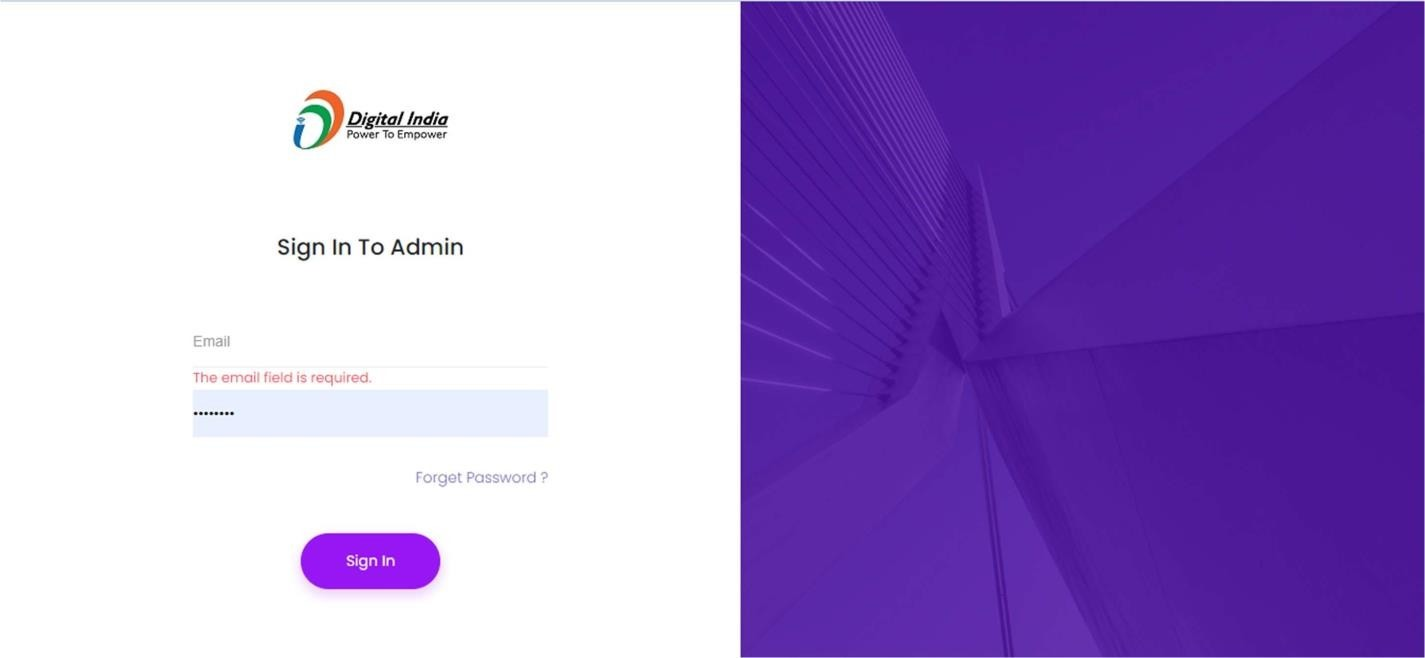
\includegraphics[height=9cm,width=14cm]{Admin/TC01}
\end{center}

\textbf{Test Case 02}
\begin{center}
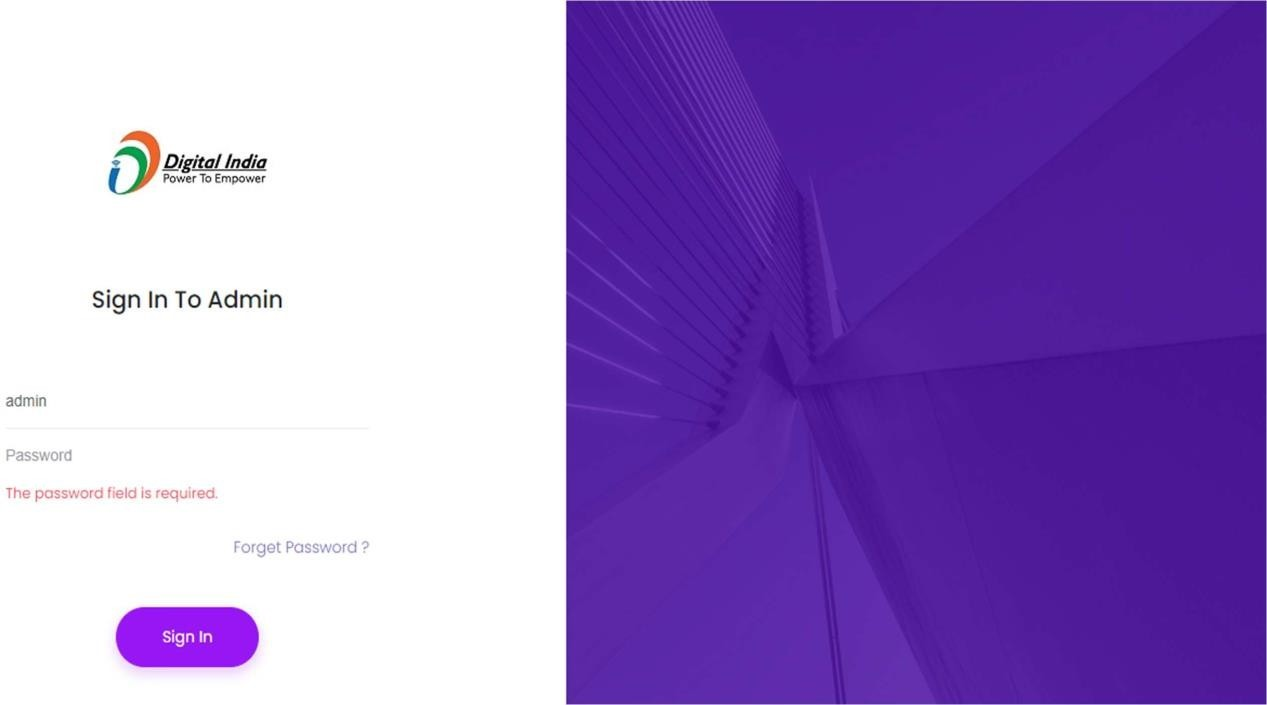
\includegraphics[height=9cm,width=14cm]{Admin/TC02}
\end{center}
\pagebreak

\textbf{Test Case 03}
\begin{center}
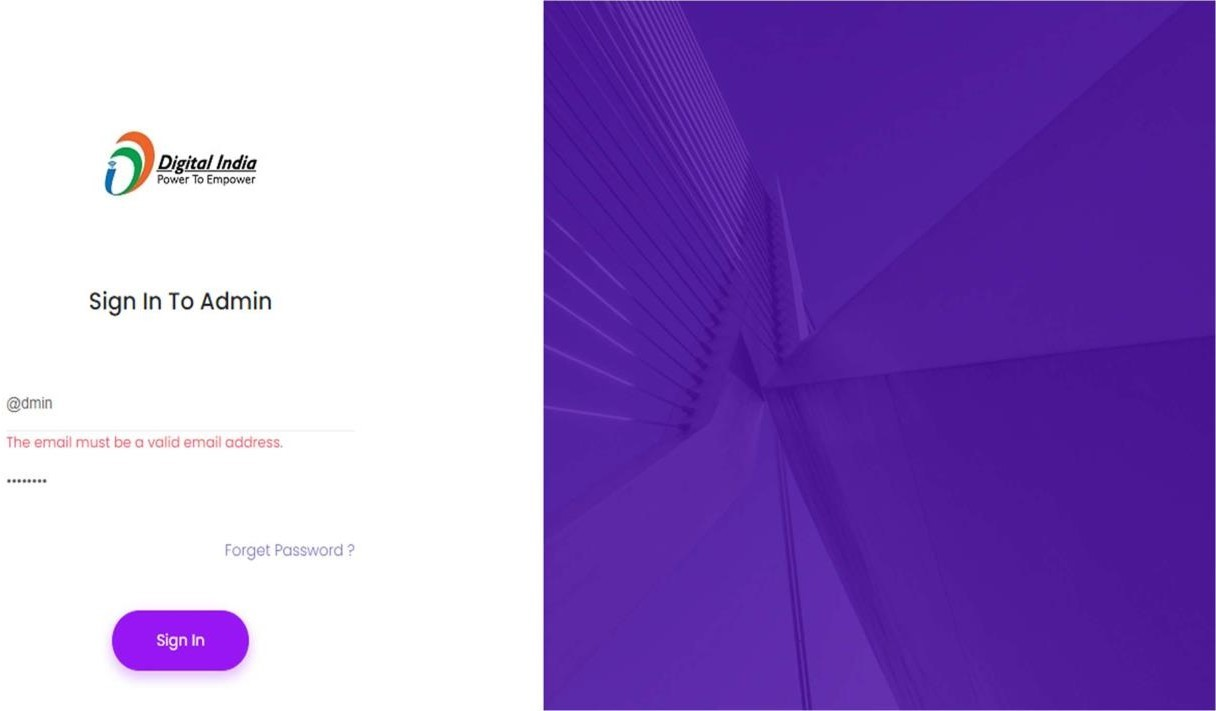
\includegraphics[height=9cm,width=14cm]{Admin/TC03}
\end{center}

\textbf{Test Case 04}
\begin{center}
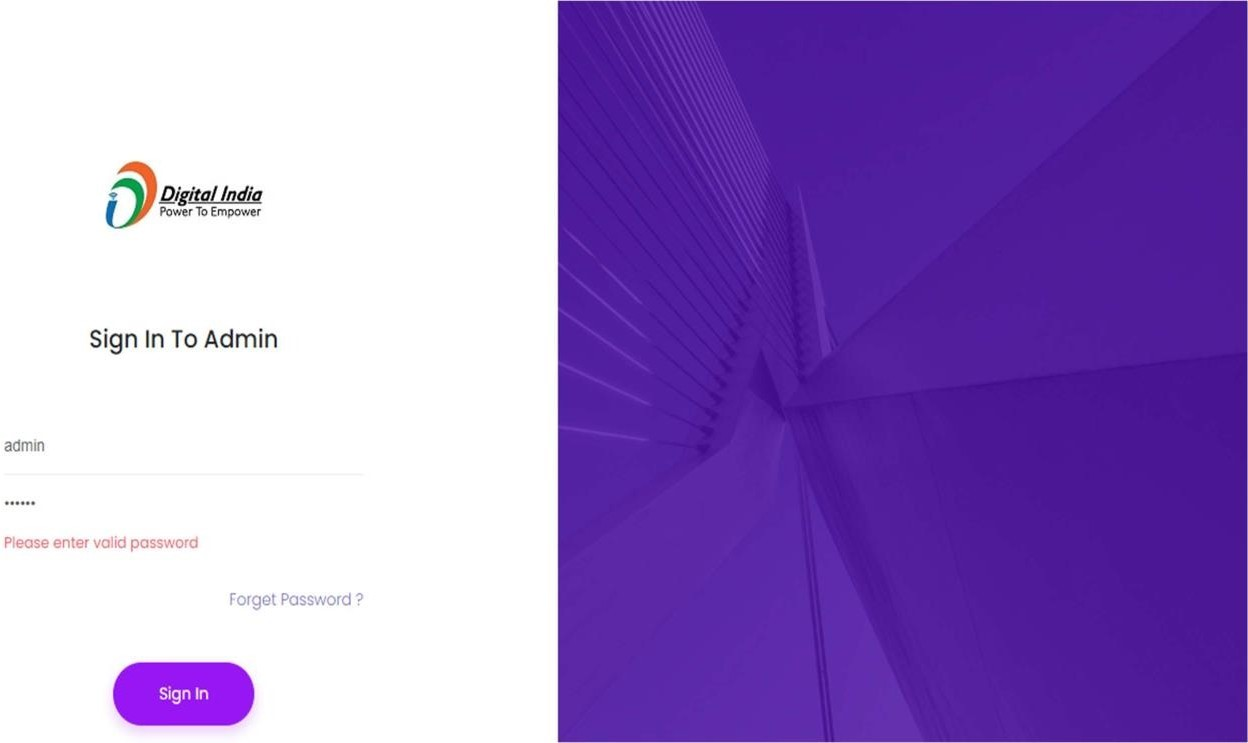
\includegraphics[height=9cm,width=14cm]{Admin/TC04}
\end{center}
\pagebreak

\textbf{Test Case 05}
\begin{center}
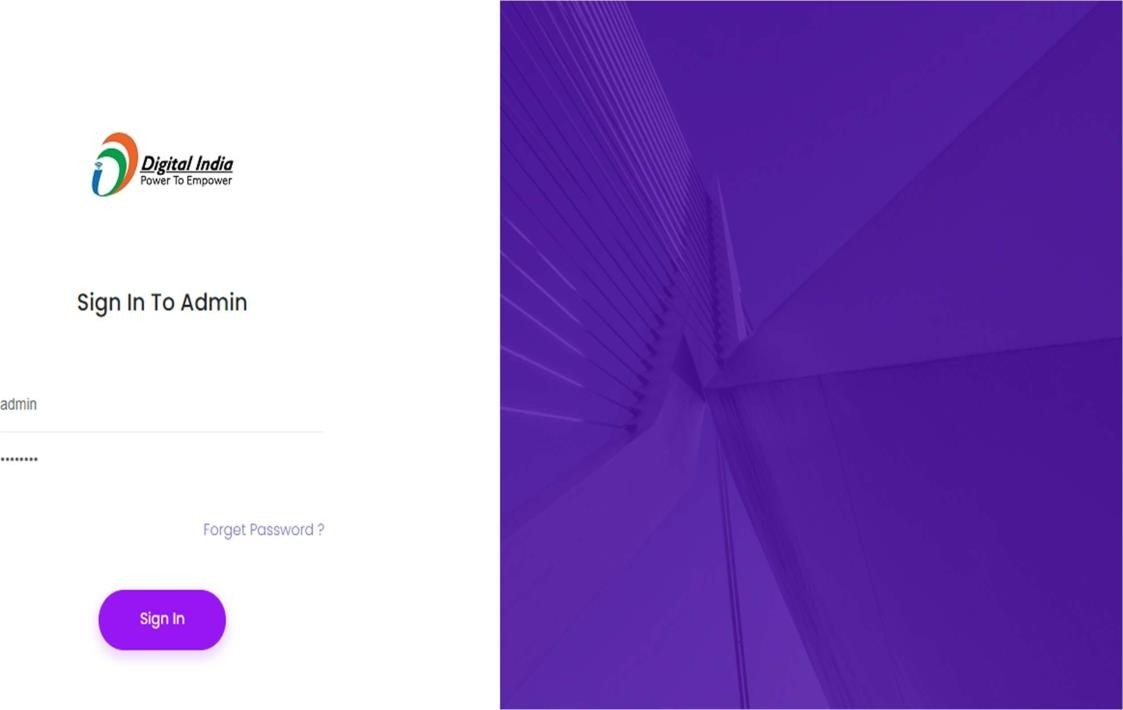
\includegraphics[height=9cm,width=14cm]{Admin/TC05}
\end{center}

% This section type your project contents 
\chapter{Concluding Remarks}


\section{Strengths of System}

Smart home automation allows you to tap into hightech functionality and luxury that wasn’t possible in the past. As technology development continues to expand, so will the possibilities for consumer home automation to make life easier and more enjoyable.




% This section type your project contents 

\section{Limitations of system}

\begin{itemize}
\item  While the potential for remote device tampering is plenty scary, it pales in comparison with the risk of a physical break-in posed by security devices like
smart door locks and surveillance cameras.
\item  Not only do these digital voice assistants listen in on you continuously while on, but hackers can also exploit security loopholes to break into the speaker and issue their own commands or harvest prior recordings.
\item  The data transmitted by smart devices like printers and smart TVs are often unencrypted, a virtual villain can view—and alter—data collected by your devices.


% This section type your project contents 
\end{itemize}

\section{Scope for future development} 

In future we add User module and Client Module.
The next step would be to extend this system to automate a large-scale environment, such as offices and factories.
We will set timer for the module which you want to control automatically.
Sensors in smart homes will turn off utilities, close windows, monitor security,
and report to homeowners in real time.
The smart clock will scan your schedule and adjust the bussing time that you
will get ready for the tasks which you will going to perform.


% This section type your project contents 

\section{Conclusion}

\begin{itemize}
\item	igital India’s main purpose is to create a MERN application that helps Customers and other people use their home appliances remotely using their remotely held devices like Mobile phones, tablets, etc
\item	 The main motive of learning and acquiring the skills has also been achieved. \\
o	Way of analyzing the system.\\

% This section type your project contents 
o	Importance and skill of proper database design.\\
o	Proper use of state management tools.\\

% This section type your project contents 

\item	Company too is satisfied with the quality of work.

\end{itemize}
%\addcontentsline{toc}{chapter}{References}


%\chapter*{Appendix}

% Students are write appendix then write here., Otherwise Comment this chapter in chapter list (Select main.tex file and comment in front of appendix chapter)


\addcontentsline{toc}{chapter}{Appendix}
%\textbf{\centerline{Appendix}}	\\
\chapter*{\centerline{Appendix}}
\newpage
   % Not required then comment only 
\addcontentsline{toc}{chapter}{References}
\renewcommand\bibname{References}
\begin{thebibliography}{99}



% This section type your project contents 


\bibitem{Books} Books Referred,\\
Following books proved to be very helpful during the development of the system.\\
•	CodeIgnitor for Rapid React Application Developement\\
David Upton\\
•	Software Engineering: A Practitioner’s Approach, Seventh Edition
Roger S. Pressman\\
\bibitem{Web} WebSites Visited :-\\
Following websites proved to be very helpful during the development of the system.\\
•	www.msdn.microsoft.com\\
•	www.w3schools.com\\
•	www.codeproject.com\\


% This section type your project contents 

\bibitem{diagrams} Software Used for Diagrams\\
•	Pacestar UML Diagrammer 6

% This section type your project contents 
\bibitem{SoftEng} Software Engineering a Practitioner’s Approach. (McGraw Hill Publication) 		Roger S. Pressman.
% This section type your project contents 
\end{thebibliography}
% ---------------------------------------------------------------------------------
% if any table wants to add in any chapter use following
%
%			\begin{table}[!ht]
%			\caption{Initial Testing Without Samples }   % name of table to be displayed above 						%											 				   table and in List of tables
%			\begin{tabular}{ c  c  c  c }				% table having 4 column
%							1 & 10 & 20 & 30 \\ 		% entries of column can separated by using &
%							2 & 40 & 50 & 60 \\ 		
%			\end{tabular}
%			\label{result1}		% for calling table no. in text
% 			\end{table} 
%
% ---------------------------------------------------------------------------------
\end{spacing}
\end{document}
